\section{Experiment}
\newcommand{\citeInTab}[1]{}

We demonstrate the efficiency and effectiveness of our proposed approach with experiments on three datasets: the synthetic dataset D-NeRF~\cite{D-NeRF} with 8 scenes, the real-world dataset HyperNeRF ~\cite{Nerfies} and NeRF-DS~\cite{NeRF-DS}. 
For all experiments, we report the following metrics: PSNR, SSIM~\cite{SSIM}, MS-SSIM,  LPIPS~\cite{LPIPS}, size (rendering resolution), and FPS (rendering speed). 
All experiments are conducted on one NVIDIA V100 GPU with 32GB memory.


Regarding the baselines, we compare our method against the state-of-the-art methods that are the most relevant to our work, including: D-NeRF~\cite{D-NeRF}, TiNeuVox~\cite{TiNeuVox}, Tensor4D~\cite{Tensor4D}, K-Palne~\cite{KPlanes},  HexPlane~\cite{HexPlane}, TI-DNeRF~\cite{TI-DNeRF}, NeRFPlayer~\cite{NeRFPlayer}, 4D-GS~\cite{RealTime4DGS}, Deformable 3D GS(D-3D-GS)~\cite{Deformable3DGS} and original 3D Gaussians (3D-GS). 


\subsection{Synthetic Dataset}

\begin{table}[t]
    \centering
    \caption{Quantitative comparison on D-NeRF~\cite{D-NeRF}. The \colorTop[1]{best} and \colorTop[2]{second best} results are highlighted. `-' denotes that the metric is not reported in their works. Lego is excluded.}
    \label{tab:D-NeRF-avg}
    \resizebox{1.0\linewidth}{!}{
    \setlength{\tabcolsep}{2pt}
    \begin{tabular}{c|*{5}{c}}
        \toprule
        Methods & PSNR$\uparrow$ & SSIM$\uparrow$ & LPIPS$\downarrow$ & Size & FPS$\uparrow$ \\ \midrule
        D-NeRF\citeInTab{DNeRF} & 31.14 &  0.9761 & 0.0464 & $400\times 400$ & $<1$   \\
        TiNeuVox-B\citeInTab{TiNeuVox} & 32.74  & 0.9715 & 0.0495 & $400\times 400$ & $\sim$ 1.5 \\
        Tensor4D\citeInTab{Tensor4D} & 27.44 &  0.9421  &  0.0569 & $400\times 400$ & -\\
        KPlanes\citeInTab{KPlanes} & 31.41 & 0.9699  & 0.0470 & $400\times 400$ & $\sim$ 0.12 \\
        HexPlane-Slim\citeInTab{HexPlane} & 32.97 & 0.9750 & 0.0346 & $400\times 400$ & 4 \\
        Ti-DNeRF\citeInTab{TI-DNeRF} & 32.69 & 0.9746 & 0.358 & $400\times 400$ & -  \\
        \midrule
        3D-GS\citeInTab{3D-GS} & 23.39 & 0.9293 & 0.0867 & $800\times 800$ & \colorTop[2]{184.21} \\
        4D-GS\citeInTab{4D-GS} & 35.31  & 0.9841  & \colorTop[2]{0.0148}  & $800\times 800$ & 143.69 \\
        D-3D-GS\citeInTab{Deformable3DGS} & \colorTop[1]{40.23} & \colorTop[1]{0.9914} & \colorTop[1]{0.0066} &
        $800\times 800$ & 45.05 \\
        \textbf{SP-GS(ours)} & 37.98  & 0.9876  & 0.0185 & $800\times 800$ & \colorTop[1]{227.25} \\
        \textbf{SP-GS+NG(ours)} & \colorTop[2]{38.28}  & \colorTop[2]{0.9877}   & 0.0152 & $800\times 800$ & 119.35  \\
        \bottomrule
    \end{tabular}
    }
\end{table}

\begin{figure*}[t]
    \centering
    \includegraphics[width=0.9\linewidth]{pics/DNeRF_results.pdf}
    \caption{Qualitative comparisons of baselines and our method on D-NeRF~\cite{D-NeRF}.}
    \label{fig:cmp-D-NeRF}
\end{figure*}

The D-NeRF dataset consists of 8 videos, each containing 50-200 frames. The frames together with camera pose serve as the training data, while test views are taken from novel views.
Quantitative and qualitative results are shown in Tab.\ref{tab:D-NeRF-avg} and Fig.\ref{fig:cmp-D-NeRF}. Though rendered at a resolution of $800\times 800$, we achieved a much higher FPS than previous non-Gaussian-Splatting based methods. As for D-3D-GS, they directly apply a deformation network to every single 3D Gaussian for a higher visual quality, leading to a much lower FPS than ours. We achieve superior or comparable results against previous state-of-the-art methods in terms of all metrics. It's noteworthy that Lego is excluded while calculating the metrics as we observed a discrepancy in all methods. Please refer to Fig. \ref{fig:cmp-D-NeRF} for a visualized results.
Per-scene comparisons are provided in Appendix \ref{sec-ap:DNeRF-results}.


\subsection{Real-World Dataset}

The HyperNeRF dataset~\cite{Nerfies} and NeRF-DS~\cite{NeRF-DS} serve as two real-world benchmark dataset captured using either one or two cameras. For a fair comparison with previous methods, we use the same \textit{vrig} scenes, a subset of the HyperNeRF dataset.
Quantitative and qualitative results of the HyperNeRF dataset are shown in Tab.\ref{tab:HyperNeRF-avg} and Fig.\ref{fig:cmp-HyperNeRF}, while results of NeRF-DS are shown in Tab. \ref{tab:NeRF-DS} and Fig. \ref{fig:cmp-NeRF-DS}. As shown in Tab. \ref{tab:HyperNeRF-avg} and Tab. \ref{tab:NeRF-DS}, our method outperforms baselines by a large margin in terms of FPS while achieving a superior or comparable visual quality. As shown in Fig.\ref{fig:cmp-HyperNeRF}, our results exhibit notably higher visual quality, particularly in the hand area.


\begin{figure*}[t]
    \centering
    \setlength{\tabcolsep}{1pt}
    \begin{tabular}{*{7}{c}}
    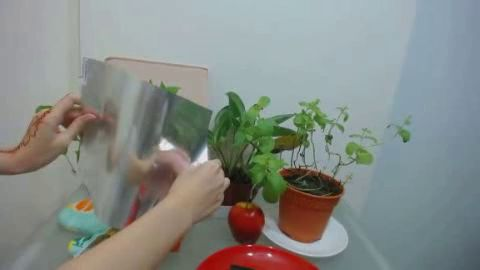
\includegraphics[width=0.14\linewidth]{pics/NeRF_DS/as_GT_245.jpg} & 
    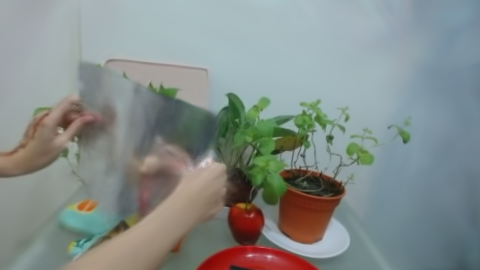
\includegraphics[width=0.14\linewidth]{pics/NeRF_DS/as_ours.png} &
    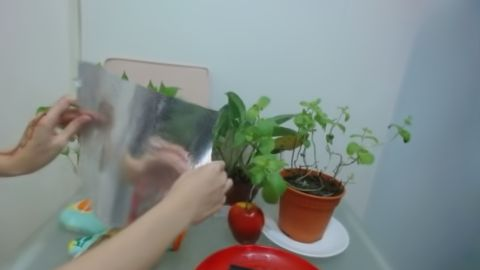
\includegraphics[width=0.14\linewidth]{pics/NeRF_DS/as_D_3D_GS.jpg} &
    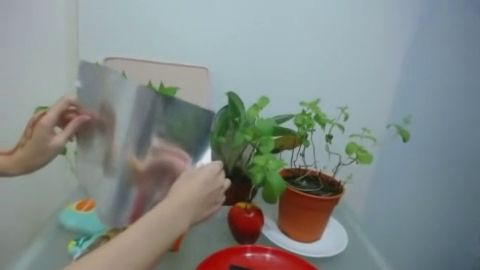
\includegraphics[width=0.14\linewidth]{pics/NeRF_DS/as_NeRF_DS.jpg} &
    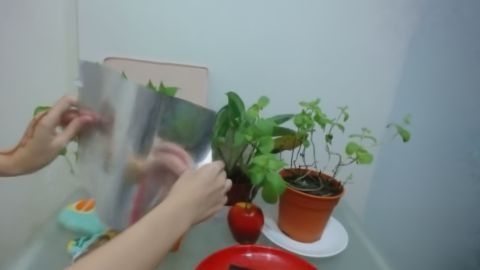
\includegraphics[width=0.14\linewidth]{pics/NeRF_DS/as_HyperNeRF.jpg} &
    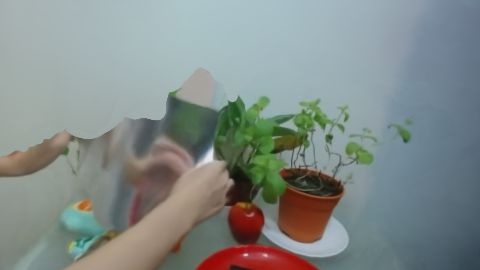
\includegraphics[width=0.14\linewidth]{pics/NeRF_DS/as_TiNeuVox.jpg} &
    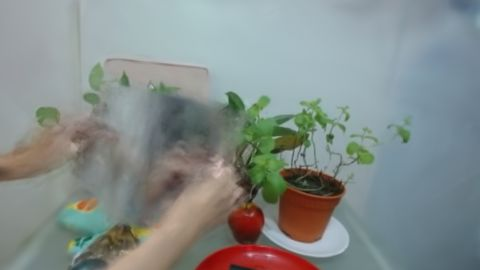
\includegraphics[width=0.14\linewidth]{pics/NeRF_DS/as_3D_GS.jpg} 
    \\
    GT & \textbf{SP-GS(ours)} & D-3D-GS & NeRF-DS & HyperNeRF & TiNeuVov & 3D-GS\\ 
    \end{tabular}
    \caption{Qualitative comparisons of baselines and our method on NeRF-DS dataset~\cite{NeRF-DS}.}
    \label{fig:cmp-NeRF-DS}
\end{figure*}

\begin{figure*}[t]
    \centering
    \setlength{\tabcolsep}{1pt}
    \begin{tabular}{*{8}{c}}
    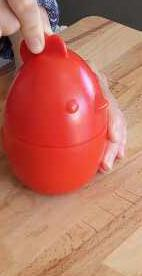
\includegraphics[width=0.12\linewidth]{pics/HyperNeRF/gt.jpg} & 
    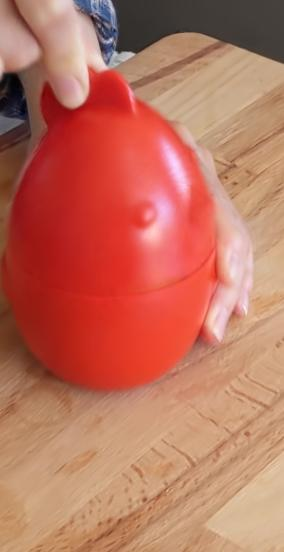
\includegraphics[width=0.12\linewidth]{pics/HyperNeRF/ours.jpg} & 
    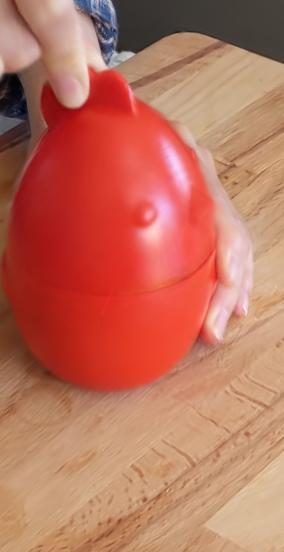
\includegraphics[width=0.12\linewidth]{pics/HyperNeRF/ours_NG.jpg} & 
    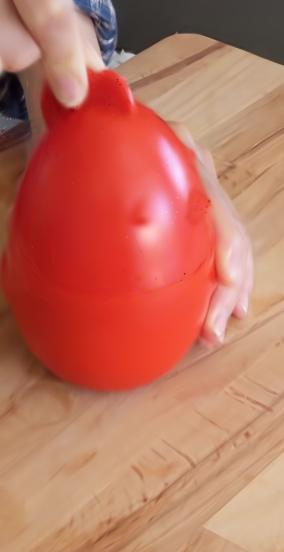
\includegraphics[width=0.12\linewidth]{pics/HyperNeRF/4D_GS.jpg} & 
    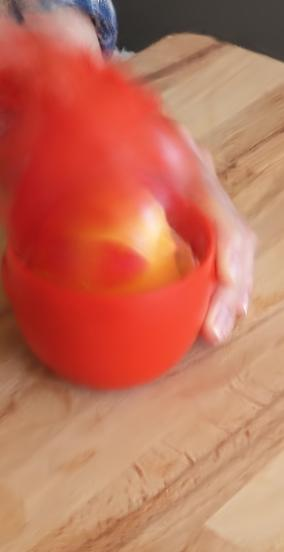
\includegraphics[width=0.12\linewidth]{pics/HyperNeRF/3D_GS.jpg} & 
    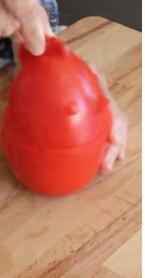
\includegraphics[width=0.12\linewidth]{pics/HyperNeRF/nerplayer.jpg} & 
    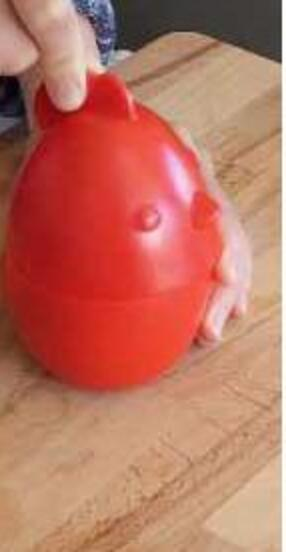
\includegraphics[width=0.12\linewidth]{pics/HyperNeRF/hyperNeRF.jpg} & 
    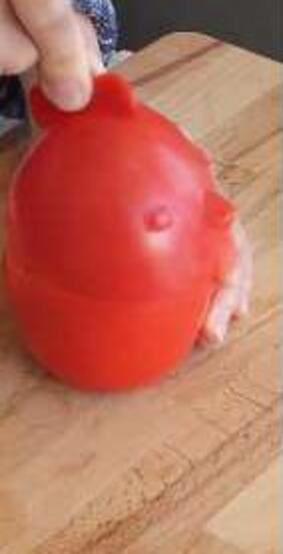
\includegraphics[width=0.12\linewidth]{pics/HyperNeRF/nerfies.jpg} 
    \\
    GT & \textbf{SP-GS (ours)} & \textbf{SP-GS+NG} & 4D-GS & 3D-GS &  NeRFPlayer &  HyperNeRF & Nerfies 
    \end{tabular}
    \caption{Qualitative comparisons of baselines and our method on HyperNeRF dataset\cite{HyperNeRF}.}
    \label{fig:cmp-HyperNeRF}
\end{figure*}

\begin{table}[t]
    \centering
    \caption{Quantitative comparison on HyperNeRF dataset~\cite{HyperNeRF}. The \colorTop[1]{best} and \colorTop[2]{second best} results are highlighted. `-' denotes that the metric is not reported in their works.}
    \label{tab:HyperNeRF-avg}
    \resizebox{\linewidth}{!}{
    \setlength{\tabcolsep}{2pt}
    \begin{tabular}{*{6}{c}}
        \toprule
        Methods  & PSNR$\uparrow$ & MS-SSIM  $\uparrow$ & LPIPS  $\downarrow$ & Size &  FPS $\uparrow$  \\ \midrule
        Nerfies\citeInTab{Nerfies} & 22.2 & 0.803 & - & $536\times 960$ & $< 1$ \\
        HyperNeRF\citeInTab{HyperNeRF} & 22.4 & 0.814 & -&$536\times 960$ & $< 1$  \\
        TiNeuVox-S \citeInTab{TiNeuVox} & 23.4 & 0.813 & -& $536\times 960$ & $< 1$ \\
        TiNeuVox-B \citeInTab{TiNeuVox}  & 24.3 & 0.837 & - & $536\times 960$ &  $< 1$  \\
        TI-DNeRF\citeInTab{TI-DNeRF} & 24.35 & \colorTop[2]{0.866} && $536\times 960$ & $< 1$\\
        NeRFPlayer\citeInTab{NeRFPlayer} & 23.7 & 0.803 & - & $536\times 960$ & $< 1$\\
        \midrule
        3D-GS \citeInTab{3D-GS} & 20.26 &  0.6569 & 0.3418 &$536\times 960$ & \colorTop[2]{71}  \\
        4D-GS \citeInTab{4D-GS}  &  25.02 &  0.8377 &  0.2915
& $536\times 960$ & 66.21   \\
        \textbf{SP-GS (ours)} & \colorTop[2]{25.61} & 0.8404  & \colorTop[2]{0.2073} &$536\times 960$ & \colorTop[1]{117.86} \\
        \textbf{SP-GS+NG (ours)} & \colorTop[1]{26.78} & \colorTop[1]{0.8920} & \colorTop[1]{0.1805} &$536\times 960$ & 51.51\\
        \bottomrule
    \end{tabular}
    }
\end{table}

\begin{table}[t]
    \centering
    \caption{Quantitative comparison on NeRF-DS~\cite{NeRF-DS}. The rendering size is $480 \times 270$.
    }
    \label{tab:NeRF-DS}
    \resizebox{\linewidth}{!}{
    \setlength{\tabcolsep}{2pt}
    \begin{tabular}{c*{5}{c}}
    \toprule
      Methods   & PSNR$\uparrow$ & SSIM$\uparrow$ & LPIPS(VGG)$\downarrow$ & FPS$\uparrow$ \\ \midrule
    TiNeuVox       & 21.61 & 0.8241 & 0.3195 & - \\
    HyperNeRF      & 23.45 & 0.8488 & 0.2002 & - \\
    NeRF-DS        & 23.60 & 0.8494 & 0.1816 & - \\ 
    \midrule
    3D-GS          & 20.29 & 0.7816 & 0.2920 & 185.43 \\ 
    D-3D-GS & 24.11 & 0.8525 & 0.1769 & 15.27 \\
\textbf{SP-GS(ours)} & 23.15 & 0.8335 & 0.2062 & 251.70 \\
\textbf{SP-GS+NG(ours)} & 23.33 & 0.8362  & 0.2084 & 66.13\\
    \bottomrule
    \end{tabular}
    }
\end{table}


\subsection{Ablation Study}
In our paper, we introduce two hyperparameters: the number of superpoints and the number of nearest neighborhoods $\mathcal{N}_i$. We conduct experiments on testing how sensitive our method is to the variation of the two hyperparameters. 
Tab. \ref{tab:as_num} shows the performance of our approach when varying these hyperparameters, and our method appears to be robust under all these variations. 
Besides, we introduce property reconstruction loss to facilitate grouping similar Gaussians together. Tab. \ref{tab:property-loss} demonstrates that property reconstruction loss can improve rendering quality.
We provide more ablations on property reconstruction loss in Appendix.\ref{sec-ap:more-exp}.


\subsection{Visualization of 3D Gaussians and Superpoints}
As depicted in Fig. \ref{fig:vis}, we provide a visualized result of the 3D Gaussians and superpoints for the hook scene of D-NeRF~\cite{D-NeRF}. Notably, we observe that the superpoints are uniformly distributed in the space while nearby 3D Gaussians will be aggregated into one superpoint. 
For a more intuitive understanding, readers can refer to our \href{https://dnvtmf.github.io/SP_GS.github.io/}{project page} for more videos.

\begin{figure}[t]
    \centering
    \subfigure[]{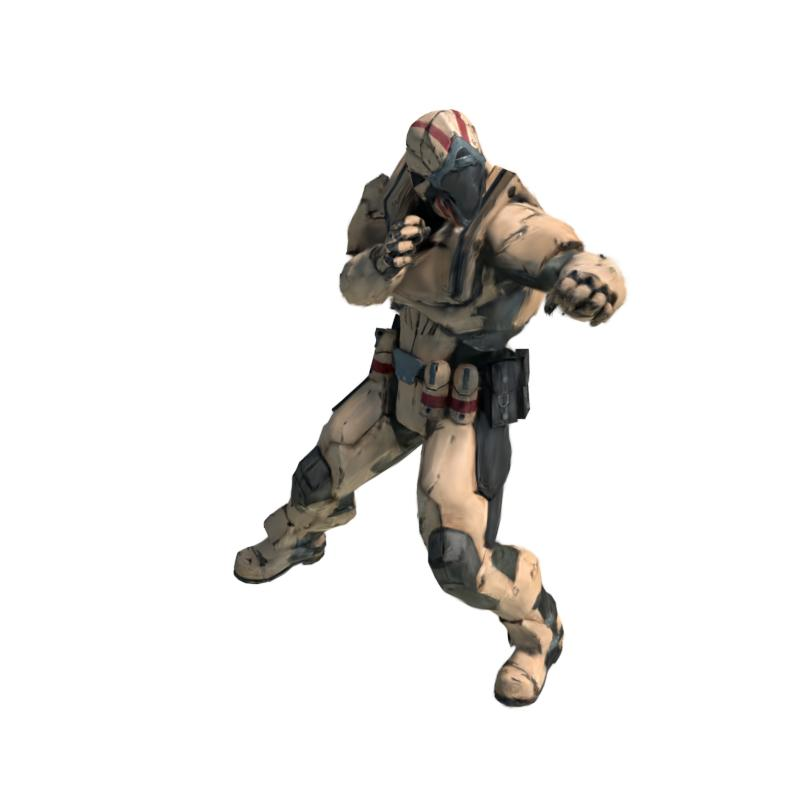
\includegraphics[width=0.24\linewidth, trim=50 50 50 50,clip]{pics/rendering.jpg}}
    \subfigure[]{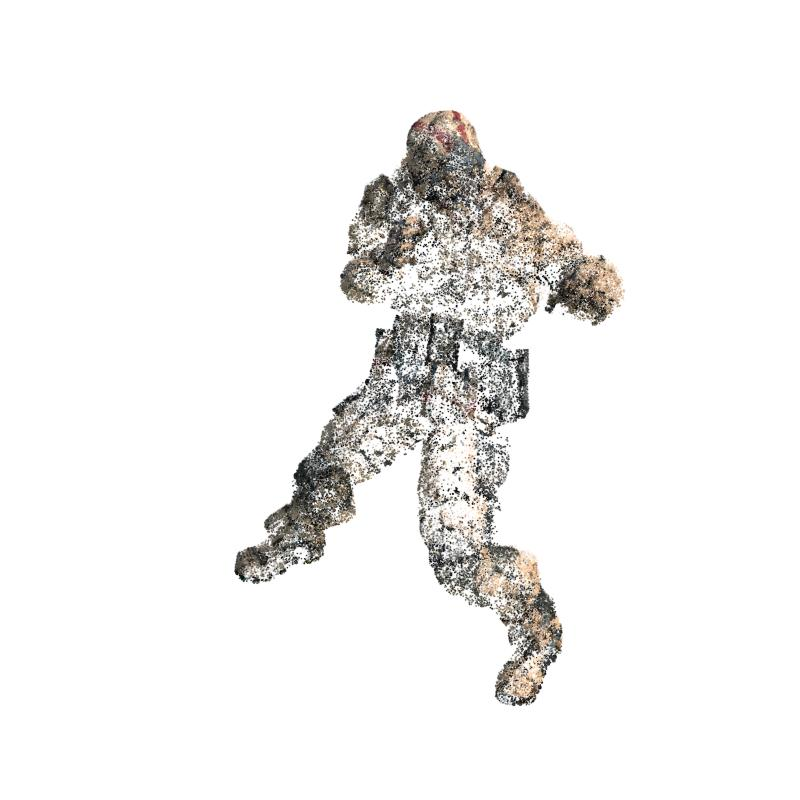
\includegraphics[width=0.24\linewidth, trim=50 50 50 50,clip]{pics/points.jpg}}
    \subfigure[]{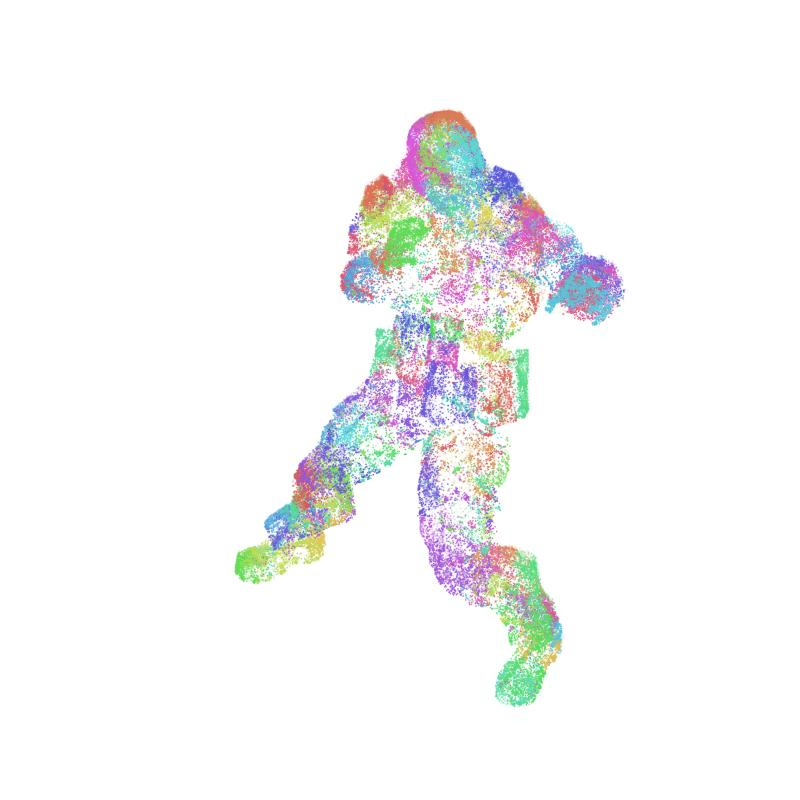
\includegraphics[width=0.24\linewidth, trim=50 50 50 50,clip]{pics/colored.jpg}}
    \subfigure[]{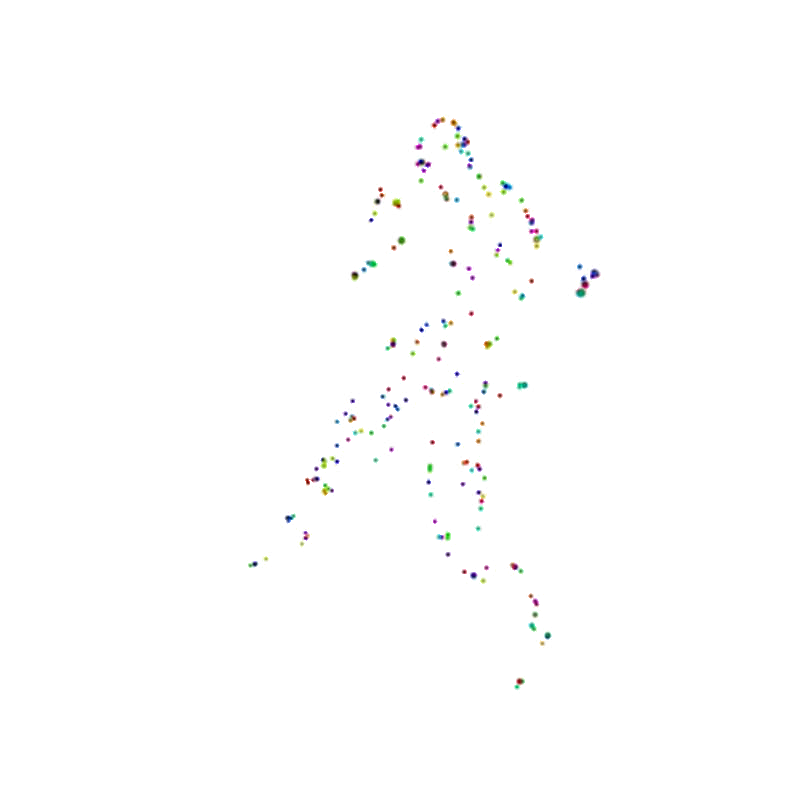
\includegraphics[width=0.24\linewidth, trim=50 50 50 50,clip]{pics/superpoints.png}}
    \caption{We visualize 3D Gaussians and superpoints by simply coloring the correspondent points. (a) the rendered image. (b) 3D Gaussians with its original color. (c) 3D Gaussians colored by superpoints, which means 3D Gaussians in one superpoint will be the same color. (d) the superpoints.}
    \label{fig:vis}
\end{figure}

\begin{table}[t]
    \centering
    \caption{Ablation Study for the number of superpoints (\#sp) and nearest neighborhoods (\#knn) on D-NeRF dataset.}
    \label{tab:as_num}
    \resizebox{0.9\linewidth}{!}{
        \begin{tabular}{c*{6}{c}}
            \toprule
        \#sp & 50 & 100 & 200 & 300 & 400 & 500  \\
        \midrule
        PSNR$\uparrow$ & 35.69 & 36.00 & 36.31 & 36.43 & 36.36 & 36.52\\ \bottomrule
        \#knn & 1 & 2 & 3 &4 &5&6\\ \midrule
        
        PSNR$\uparrow$ &36.24 & 36.11 & 36.09 & 36.09 & 36.30 & 36.23 \\ \bottomrule
        \end{tabular}
    }
\end{table}

\begin{table}[t]
    \centering
    \caption{Ablation study for property reconstruction loss on D-NeRF dataset.}
    \label{tab:property-loss}
    \begin{tabular}{cccc}
        \toprule
        Method & PSNR$\uparrow$ & SSIM$\uparrow$ & LPIPS$\downarrow$ \\ \midrule
        w/o loss & 37.59 & 0.9868 &  0.0172\\
w loss	& 37.98 & 0.9876 & 0.0164  \\ \bottomrule     
    \end{tabular}
\end{table}

\begin{table}[t]
    \centering
    \caption{The results of distillation on ``As" scene of NeRF-DS dataset. We use D-3D-GS as teacher model, and use SP-GS as student model.}
    \label{tab:distill}
    \setlength{\tabcolsep}{1pt}
    \resizebox{\linewidth}{!}{
        \begin{tabular}{*{6}{c}}
            \toprule
            Method & PSNR$\uparrow$& MS-SSIM $\uparrow$ & LPIPS$\downarrow$ & FPS$\uparrow$  \\ \midrule
            teacher (D-3D-GS) & 26.15 & 0.8816 & 0.1829 & 20.65\\
            student (SP-GS) & 25.68 & 0.8811 & 0.1982 & 164.04 \\
            ours (SP-GS) & 	24.44 & 0.8626 & 0.2255 & 250.32 \\
            \bottomrule
        \end{tabular}
    }
\end{table}

\begin{figure}[thb]
    \centering
    \subfigure[Pose Estimation]{\label{fig:repose}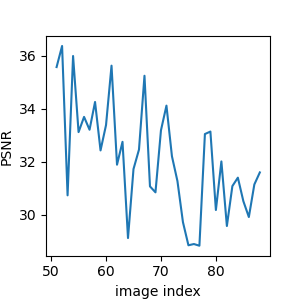
\includegraphics[width=0.48\linewidth]{pics/pose.png}}
    \subfigure[Scene Editing]{\label{fig:edit} 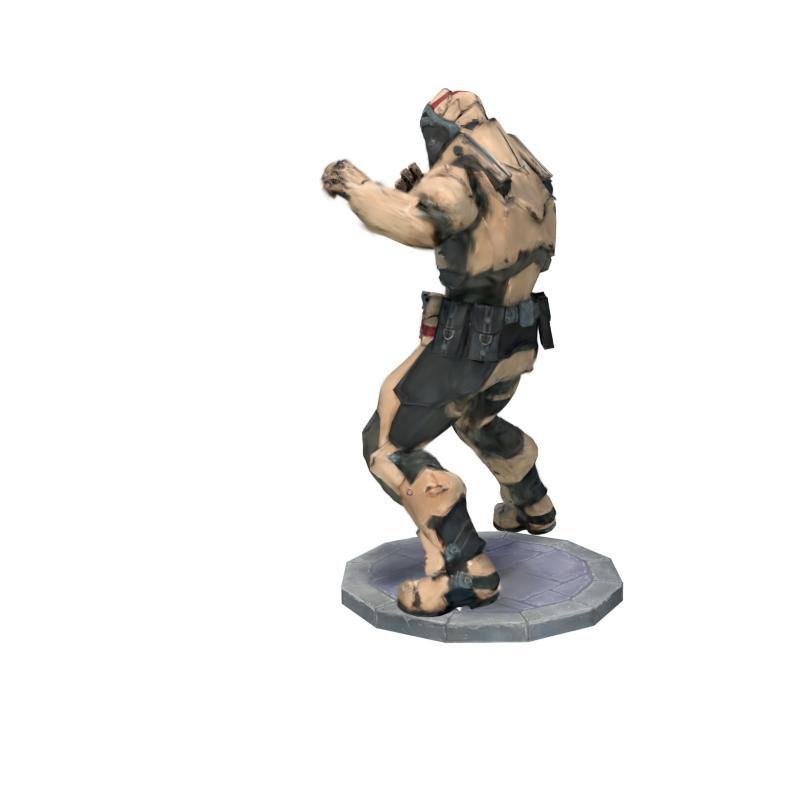
\includegraphics[width=0.48\linewidth]{pics/edit.jpg}}
    \caption{(a) The PSNR results for pose estimation results on the jumpingjacks scene. (b) We add the base of the trex scene to the bottom of the hook scene.}
    \label{fig:app}
\end{figure}